\documentclass[conference]{IEEEtran}
\IEEEoverridecommandlockouts
\usepackage{cite}

\usepackage{tcolorbox}
\usepackage[colorinlistoftodos,prependcaption]{todonotes}
\usepackage{xcolor}
\usepackage{amsmath,amssymb,amsfonts}
\usepackage{algorithmic}
\usepackage{graphicx}
\usepackage{textcomp}
\usepackage{minted}
\usepackage{subcaption}
\usepackage[hidelinks]{hyperref}
\usepackage[inline]{enumitem}
\usepackage[T1]{fontenc}
\usepackage{cleveref}
\usepackage{systeme}
\setminted[scala]{baselinestretch=1,bgcolor=white,frame=single}

\def\BibTeX{{\rm B\kern-.05em{\sc i\kern-.025em b}\kern-.08em
  T\kern-.1667em\lower.7ex\hbox{E}\kern-.125emX}}
\sloppy



\newcommand{\unibo}{\textsc{Alma Mater Studiorum} -- \textit{Università di Bologna}}
\newcommand{\disi}{\textit{Computer Science and Engineering - DISI}}
\newcommand{\scafi}{{ScaFi}}
\newcommand{\scalaloci}{{ScalaLoci}}
\newcommand{\scafiloci}{{ScaFiLoci}}
\newcommand{\scalainline}[1]{\mintinline[fontsize=\small]{scala}{#1}}
%%%%% LEGENDA FOR NOTES %%%%%
%% RED: constraints
%% YELLOW: suggestions
%% CYAN: todos
%% GREEN: outline
\newcommand{\constraints}[1]{\todo[inline, color=red]{#1}}
\newcommand{\suggestions}[1]{\todo[inline, color=yellow]{#1}}
\newcommand{\todos}[1]{\todo[inline, color=cyan]{\textbf{TODO}: #1}}
\newcommand{\outline}[1]{\todo[inline, color=green]{#1}}
%% Utility commands
\newcommand{\hybridaggregate}{\textit{Hybrid Aggregate Computing}}
\newcommand{\round}{\texttt{round}}
\newcommand{\export}{\texttt{export}}

\begin{document}

\title{Towards a Machine Learning approach for Aggregate Computing} %% or Towards a Machine Learning approach for Aggregate Computing
\author{\IEEEauthorblockN{
Gianluca Aguzzi\IEEEauthorrefmark{1},
Roberto Casadei\IEEEauthorrefmark{1},
Mirko Viroli\IEEEauthorrefmark{1}
}\\
\IEEEauthorblockA{\IEEEauthorrefmark{1}
\textsc{Alma Mater Studiorum}---Universit\`a di Bologna, Cesena, Italy\\
Email: \{gianluca.aguzzi, roby.casadei, mirko.viroli\}@unibo.it
}}

%% Minted helpers
\definecolor{mblue}{rgb}{0.27,0.33,0.53}
%%
%% Keywords. The author(s) should pick words that accurately describe
%% the work being presented. Separate the keywords with commas.
%\begin{keywords}
%  Collective-Adaptive System \sep
%  Aggregate Computing \sep
%  Deep Learning \sep
%  Reinforcement Learning \sep
%\end{keywords}

%%
%% This command processes the author and affiliation and title
%% information and builds the first part of the formatted document.

\maketitle
\begin{abstract}
Artificial intelligence is here to stay. 
 In particular, Machine Learning techniques in the last years outperform 
 hand-craft human solutions in different contexts, ranging from computer vision to videogames.
%
Currently, though, an all-encompassing Machine learning algorithm does not exist, 
 so researchers explore the possibility to apply these techniques in different fields.

One of the most challenging is Collective-Adaptive System (CAS). % Or do we want to use Cyber-Physical Swarm??
 Here, engineers have to handle large scale, global-to-local behaviour mapping,
 highly environment stochasticity. 
%
Historically, researchers favour handling them with self-organisation,
 by which a collective behaviour emerges from continuously local interaction between simple components.
%
A novel technique to specify self-organising behaviour in a composable and functional manner is Aggregate Computing.
 In particular, this paradigm enables collective program specification as a whole, 
 as it is based on a distributed data structure manipulation called \textit{computational fields}.
 It is successfully used in different scenarios ranging from Swarm Robotics to Smart cities.
 
Even though it is promising for expressing high-level collective behaviour,
 practically it is difficult to make programs work in highly dynamic networks, 
 where nodes have to deal with continuous changes at the environment side.
%
Therefore, with this work, we stand the first step towards integration between Aggregate Computing and Machine Learning,
 in order to improve adaptivity acting in the low-level specifications but maintaining the high-level program behaviours. 

In the article, we outline issues, opportunities and methodologies of this integration, presenting a case study
 where Aggregate Computing is successfully combined with Hysteretic Q-Learning.
%

\end{abstract}
\begin{IEEEkeywords}
  Collective-Adaptive System,
  Aggregate Computing,
  Deep Learning,
  Reinforcement Learning
\end{IEEEkeywords}
  
\section{Introduction}
Nowadays, computer engineers have to deal with Collective Adaptive Systems (CASs)
 due to the increasing interconnected computational devices placed in ever-changing environments.
 Examples of those include robot swarm, smart cities and augmenting crowds.

CAS are notoriously hard~\cite{DBLP:conf/huc/Ferscha15} to design as they are characterised by 
\begin{itemize}
\item a global order that emerges from local node interactions, 
\item decentralised control, and 
\item adaptive behaviours towards environmental changes to pursuit a collective goal.
\end{itemize} 
%
So, over the years, in literature, various approaches aim at handling this complexity. 
%
Some of them take inspiration from the natural system
 composed of social animals --- like bees, fish and ants. 
%
Here, a sort of hive mind arises -- 
 something referred to as swarm intelligence -- 
born from local interactions between agents. 
%
These kinds of behaviours are accomplished with self-organisation, 
 namely a global order that emerges from continuous 
 interactions between simple entities.

Initially, researchers try to bring those properties into the computer science world 
 by miming the collective behaviour bottom-up, 
 namely trying to find the right single node behaviour 
 to reach a global behaviour, e.g. flocking, foraging, etc.
%
Though, this mapping isn't easily definable ---
 since we handle complex systems.
%
Ideally, we would like to express collective behaviours focusing only at the ensemble level,
 abstracting over non-functional aspects such as the network topology, environment uncertainties and 
 so on.

In this direction, Aggregate Computing~\cite{DBLP:journals/computer/BealPV15} is an innovative solution by which 
 developers can express collective self-organising behaviours through a functional program specification.
%
Indeed, an aggregate program (i.e. a program written with Aggregate Computing) consists of the manipulation of \textit{computational fields}, a distributed
 data structure where each point in the spacetime is associated with the result of a computation
 performed by a node.
%
These operations are defined in \textit{field-calculus}~\cite{DBLP:conf/coordination/AudritoBDV18} --- the root of Aggregate Computing. 
 This calculus describes a set of minimal constructs to express any spatiotemporal computation.
%
Thanks to the ``composable'' nature of Aggregate Computing, we find common abstractions 
 in collective behaviour specification, and then we encapsulate them in so-called ``building blocks''.
%
With those, different properties have been proven (such as \textit{eventual consistency}~\cite{DBLP:journals/taas/BealVPD17}) and various
 applications have been built (such as swarm robotics, crowds engineering~\cite{DBLP:journals/eaai/CasadeiVAPD21}).

Anyway, building block synthesis concerns different stuff related not only to the behaviour itself
 but also to the "ensemble" specifications. 
 For instance, it is quite difficult to craft building blocks
 that easily adapt w.r.t the node movements rapidity.

So, we claim that Machine Learning can help us in handling this "unseen" situation, leaving only the burden
 to developers of defining the right collective specifications.
%
This lead to an ``hybrid" approach where a part of behaviour is still expressed using common 
 Aggregate Computing abstractions and another part is distilled through learning~\cite{research}.
%
In this paper, as the first steps towards a so-called \hybridaggregate{},
 we investigate how Aggregate Computing can be extended with Reinforcement Learning through a case study,
 where we outline the performance improvement of the "hop count" program.
\todos{Outline}

\section{Background and Related Work}

Computer Science is an incredibly evolving research area. 
 In a few years, the environment had been filled with intercommunicating computational devices, such as smartphones, smart things, and personal computers.

In particular, in literature, we speak of Collective Adaptive Systems
 when the number is incredibly high, there is no central authority that coordinate nodes,
 the overall behaviour is reached with local interactions, the systems expose self-* properties,
 and the ensemble pursuit of collective goals
 exhibiting swarm intelligence.
 
Engineering this kind of system is a thriving area, various approaches have been proposed.
 First attempts leverage so-called \textit{local-to-global} techniques, where the collective behaviour emerges from local behaviour description, 
 usually inspired by nature~\cite{DBLP:journals/swarm/BrambillaFBD13}. 
%
Though, a natural way to describe this kind of problem is by using an \textit{collective} view of the system.
 And it is the idea used by the \textit{global-to-local} techniques~\cite{DBLP:journals/jlap/ViroliBDACP19,DBLP:journals/scp/AlrahmanNL20, DBLP:conf/cbse/BuresGHKKP13}, where the behaviours are designed \textit{top-down},
 and then the local behaviour is generated automatically. 
% 
Also ``meet-in-the-middle''~\cite{DBLP:journals/computer/PinciroliB16} approaches exist, where
 a part of the system is still expressed bottom-up (device-centric) whereas a part is expressed top-down (swarm-centric)

In our works, we are focused on Aggregate Computing~\cite{DBLP:journals/computer/BealPV15}, global-to-local approach where
 the self-organising collective behaviour is expressed in terms of manipulation of \textit{computational fields}.

The latter could be seen as the extension of electromagnetic fields to computer science since it basically consists in a 
 map from any device to its computational value (i.e. the result of a computation).

The computational field manipulation is ruled by \textit{field calculus}, which define the constructs needed 
 any for express spatio-temporal computation~\cite{DBLP:conf/coordination/AudritoBDV18}.

The novelty of Aggregate Computing consists in its composable (functional-like) program definition: using basic constructs
 we identify the main patterns (\textit{building-blocks}) that could be reusable at the application level.

Crafting opportunistically these building-blocks is possible to verify prominent properties such as eventual consistency~\cite{DBLP:journals/taas/BealVPD17} (i.e. the ensamble behaviour is independent from the underlying network details)
 and self-stabilisation~\cite{DBLP:journals/tomacs/ViroliABDP18} (i.e. the ability of a system to recover from arbitrary changes).

Aggregate Computing is studied in various simulated scenarios (thanks to Alchemist, a meta-simulator for pervasive systems), ranging from smart cities to crowds, thanks to programming language and toolchain that support 
 this paradigm, such as ScaFi~\cite{DBLP:conf/ecoop/CasadeiV16}, FCCP~\cite{DBLP:conf/acsos/Audrito20} and Protelis~\cite{PianiniSAC2015}.

In the next sections, we show the field calculus operators that are essential to understand the case study presented,
 and then we underline how each node computes in order to follow the aggregate program specification.
\subsection{Field Calculus operators}
The main constructs that captures the essential aspects for programming self-organising systems are:
\begin{itemize}
  \item \textit{Stateful field evolution} expression \mintinline[escapeinside=||]{scala}{|{\color{teal}rep}|(|$e_1$|) {|($x$) => $e_2$|}} describes a field evolving in time. 
  $e_1$ is the initial field value and the function $(x) => e_2$ define how the field changes at each execution.
  \item \textit{Neighbour interaction} expression \mintinline[escapeinside=||]{scala}{|\color{teal}nbr|{|$e$|}} a view
  of the field values in the surroundings of each device where neighbours are
  mapped to their evaluations of $e$. A series of \mintinline{scala}{*hood} operators leverage this map to produce relevant result. 
  For instance, $minHood$ return the minimum value 
  from the neighbourhoods.
  \item \textit{Domain partitioning} expression \mintinline[escapeinside=||]{scala}{|\color{teal}if|(|$e_0$|){|$e_1$|}{|$e_2$|}} splits the computational
  field into two non-communicating zones hosting isolated subcomputations:
  $e_1$ where $e_0$ is true, and $e_2$ where $e_0$ is false.
\end{itemize}
\subsection{Computational Model}
An aggregate program execution consists of a continuously node-point execution of a \round{}, 
 that is the atomical part of aggregate computing.
%
Each node can interact only with-in its neighbourhoods sharing the \export{}, 
 namely the result produced by the evaluation of a \round{}.

The main round steps consist in:
\begin{enumerate}
  \item execution context creation: where node collects information from the sensors, the neighbourhoods exports and the old
  program output
  \item program evaluation: the system-wide aggregate program is evaluated against the local context created by the nodes. 
  This produces the \export{}.
  \item export sharing: the export created will be shared within the current neighbourhoods perceived by the nodes
  \item actuations: giving the export produced, nodes may perform some actuation (e.g. motor activations, steering, ...)
\end{enumerate}

Rounds execution is completely asynchronous, so do not exist a global clock to coordinate the aggregate. 
 This makes it possible to scale easily with the node number size.

This collective, proactive and periodical execution will eventually reach the system-wide specification.

\section{Aggregate computing and Machine learning}

In this section,
 we analyse the characteristics of the aggregate computing paradigm,
 map these to relevant machine learning contributions in literature,
 pointing out different learning perspectives about the integration of Aggregate Computing with Machine Learning,
 and summarise the analysis into a roadmap.

\paragraph{Multi-and many-agent system}
%
An aggregate system is a multi-agent system
 and, often, a \emph{many}-agent system
 where a large number (hundreds or more)
 of autonomous entities are programmed to achieve 
 some collective behaviour by means of \emph{repeated} 
 sensing, computation, communication, and actuation steps.
%
Due to the high stochasticity of the environment,
 it is almost impossible to know and
 program the optimal behaviour for all agents in advance.
 This results in the need to create intelligent agents
 so that they can learn the optimal behaviour and adapt to environmental changes.
%
In recent decades there has been an emerging trend in the use of Reinforcement Learning
 in multi-agent settings, as a powerful, robust and adaptive learning paradigm.
 Progress has been considerable and a wide range of algorithms are now available.
% to expand and references
This field is a conjunction of Game theory and Reinforcement Learning, 
 and there are several (even orthogonal) viewpoints on which researchers have been focused.

First attempts from Reinforcement Learning viewpoint, 
 goes towards a so-called \textit{conccurent/independent learning}~\cite{DBLP:journals/tsmc/BusoniuBS08} approach, 
 where each agent learn locally against the whole environment~\cite{DBLP:conf/icml/Tan93}. 
Here various approaches have been proposed,
 such as Hysteretic Q-Learning (used to reduce non-stationarity)~\cite{hysteretic-q}, 
 Lenient Learning~\cite{DBLP:journals/jmlr/WeiL16}, and Frequency Maximum Q-value.
The pro of these approaches is that their complexity does not scale up with the number of agents, 
 but, unfortunately, the learning process is extremely non-stationary and non-stable.
 Furthermore, they are heuristic and does not exist any convergence proof to a stationary state (even if practically often convergence to a stable policy).

%
The game theory viewpoint instead has tried to find techniques that achieve equilibrium such as Nash-equilibrium of Pareto optimality.
 The first works towards this direction are Nash-Q-Learning~\cite{nash-q}, Friend-or-Foe Q-learning~\cite{DBLP:conf/icml/Littman01}, Minimax-Q.
The problem there is that is used with few agents and scale hardly with the application complexity.
%
So, current emerging trends tend to leverage a so-called centralised training and decentralised execution (CTDE) approach, by which 
 agents should leverage the system-wide knowledge at training time but at runtime, they act independently~\cite{DBLP:journals/aamas/Hernandez-LealK19}.
 Most promising approaches in this direction are MAPPO~\cite{DBLP:journals/corr/abs-2103-01955}, COMA~\cite{DBLP:journals/corr/FoersterFANW17} and MADDPG~\cite{DBLP:conf/nips/LoweWTHAM17}.
 
%
 The main problem with most of the solutions available in the literature is that they consider a small number of agents (or at least test them on small games).

\paragraph{Neighbour-based or indirect (environment-mediated) interaction}
%
In aggregate systems, a device can only directly interact with neighbours.
%
Data flows may be implemented
 to support indirect communication across multiple hops;
 however, information from devices far away tends to be obsolete.
%
The environment can also be used, via stigmergy,
 for indirect communication;
 however, a device can typically only access 
  to a very local portion of the environment.
%
In other words, the system state is only \emph{partially observable}.

In practice, CTDE technique aims to solve these problems, using a \emph{global} view at training time but
 a \emph{partial view} at execution time.

Furthermore, when the system node size is very large, novel works of Mean-Field Reinforcement Learning~\cite{DBLP:conf/ijcnn/ZhouZX21} are able to
 handle learning efficiently, reasoning about agent and agent neighbourhoods.
%
\paragraph{Learning goal: collective behaviour}
%
The devices of an aggregate 
 must cooperatively learn the ``aggregate program'',
 namely the collective behaviour 
 that achieves a particular \emph{global goal}
 in a decentralised, resilient way.
%

% \paragraph{Self-organisation, swarm robotics} it is condensed it other perspective, so I think it is better to avoid this paragraph.
%
% \suggestions{You can talk about similar problem structure (i.e. the collective follow the same local behaviour)}

\paragraph{Emergent behaviour}
%
The collective behaviour of an aggregate system
 \emph{emerges} 
 from a dense network of computations and interactions
 in an evolving environment.
%

Typically, in CAS, single-agent RL brings to emergent behaviour and is used in various applications~\cite{DBLP:conf/icse/DAngeloGGGNPT19}.

\paragraph{Delayed, global rewards}
%
In the light of the above properties,
 if we consider a learning approach based on rewards,
 we must observe that such rewards would be
 delayed and mostly global---i.e.,
 it may not be easy to solve the credit assignment problem
 to distinguish good from bad individual contributions
 to the global outcome.

A way to handle this kind of rewards in multi-agent settings is \textit{difference rewards}~\cite{DBLP:conf/atal/DevlinYKT14}. It is used to capture agents contributions to the system's global performance.
\paragraph{Transient phase}
%
When an aggregate behaviour is carried out,
 we often focus on the stabilised outcomes,
 tolerating outcomes that are being generated
 during the transient phase.
%
However, intermediate results are often important,
 and invariants should hold throughout the entire computation.

\paragraph{Dynamic topology}
%
If we admit \emph{mobility} and \emph{failure} (rarely considered in related works, where node population is fixed),
 then we must also consider
 the possibility of changes in neighbourhoods
 and hence the need of dealing with dynamic topologies.

\subsection{Integration perspectives}
Here we outline the different perspectives about \hybridaggregate{} with the aim
 of clarifying the current research.
%
\paragraph{Application} Learning can be useful at different levels in our framework.
 Surely, what for us is most important is to improve our building blocks definition.
% 
Indeed, most of our results and applications are based on them.
%
The building block improvement may consist either of learning a correction factor or by learning the behaviour entirely.

On the other side, learning can be useful also for framework related stuff,
 mainly aim at "non-functional" aspects. 
 Trust mechanisms, evaluation frequency, energy consumption manager, package storage are all the things that could need to be handled by hand.
 
\paragraph{Learning problem} 
The learning problem in multi-agent settings can be pose as \textit{Independent} and \textit{Team} learning. 
In the foster, each agent perform the learning process and in the latter,
 the learning process is performed only by one agent and then shared with the collective.
% 
Team learning is usually used in the ``swarm'' system, due to the homogeneous behaviour 
 --- i.e. each agent performs the same program. 
 Here, a common reward signal exists and evaluate the overall collective behaviour.
 Aggregate Computing is quite near to this kind of setting.
% 
Indeed, each agent follows the \textit{same} aggregate program shared within the entire system.

On the other hand, Independent Learning is usually applied in Collective
 (Self-)Adaptive System \cite{csas-and-marl}, so again a field near to Aggregate Computing.
 In particular, Independent Reinforcement Learning seems to reach good results in this kind of system, 
 even if no theorems exist as in the single-agent context.
%
With Concurrent learning though is still possible to reach a global collective behaviour convergence. 
 Indeed using a common reward signal, the collective may reach the same behaviour \cite{iima2008swarm, nguyen2018swarm}.

\paragraph{Learning technique}
Aside from what kind of problem we set up, we can then use different Machine Learning techniques,
 such as Reinforcement Learning or Supervised Learning.
%
Supervised learning is quite rare in CSAS -- or in the ``swarm" like system in general.
%
Novel works~\cite{DBLP:conf/corl/TolstayaGPP0R19} leverage Graph Neural network to learn how agents should communicate, supposing to know the right behaviour (i.e. produced via global vision simulation).
%
In Aggregate Computing, Supervised Learning makes sense if we want to craft new building blocks by zero. 
% 
Indeed, we know eventually the right state of the system, but we do not know how the system can reach it.

Reinforcement Learning is predominantly used in CAS, 
 due to its flexibility and thanks to the plethora of approaches used in this scenario~\cite{csas-and-marl}.
% 
In our case, Reinforcement Learning can be used both at the building block level and the framework level.
%
For the foster, the simplest scenario can be that agents learn a correction factor to improve a long-term reward signal.
 
\paragraph{Learning time}
Finally, learning can be performed \textit{offline}, \texttt{online} or \textit{offine an then online} (\textit{mixed time}).
% 
The foster is the easiest scenario.
 Here indeed, we can leverage simulation to know the right computational field and then use one of the novels CTDE techniques. 
% 
Supervised, Reinforcement Learning and even Evolutionary computing can be used here.
%
Mixed-time learning can be a mid-level complexity direction instead.
 Here, simulation can always be leveraged to reach a good behaviour, but at runtime, the behaviour can be adapted in front of new environmental situations. 
%
Finally, we can imagine that learning can be performed online. 
 It is a common situation where we do not know the environment and also simulation can be very hard to accomplish. 
 
In mixed and online cases, Reinforcement Learning is the most suitable mode here --- also the "meta" learning can help.

\section{Aggregate Computing with Reinforcement}
In this section, we describe our first result in Aggregate Computing and Machine learning combination.
% 
Hence we briefly describe how Reinforcement Learning can be injected into the computation loop,
 and what kind of Reinforcement Learning can be used with Aggregate Computing.

\subsection{Reinforcement Learning integration}
From a local view, program execution can be seen as:
$$
f : \textit{Context} \rightarrow \textit{Output}
$$
Where the context contains:
\begin{itemize}
  \item $\sigma(name) \rightarrow \textit{data}$: a function from sensor name to the perceived value
  \item $\phi(\textit{ID}) \rightarrow \textit{Export}$: a function from id to neighbourhoods export data
\end{itemize}
The computational field $\theta$ contains all output produced by the system.

Speaking by Reinforcement Learning settings, we need to define the state functions and the reward functions.
%
Here the execution needs to be distributed, so the state will be a function from the local node context:
$$
K := \Omega(\textit{Context})
$$

Reward function instead, might be depending on the learning technique, time and problem. 
 Indeed, if we perform learning offline, it could be defined from the overall \textit{simulated} computational field:
$$
\textit{R}_{global} := \psi({\theta})
$$
If we use an online mode, it needs to be defined as a function to the local node context:
$$
\textit{R}_{local} := \psi(\textit{Context})
$$
Finally, actions influence the current aggregate program output, changing the program evaluation as:
$$
f_{rl} : \textit{Context} \rightarrow \lambda(\textit{Output}, \textit{Action})
$$
As remarked before, the policy $\pi$ need to be distributed, so each agent can choose the action that will be performed:
$$
\textit{Action} \leftarrow \pi(K)
$$

For our first tests, 
 we decide to set up an Independent learning technique, by which each agent try to improve our current local policy.
 Our approach is partially inspired by Swarm Q-Learning~\cite{nguyen2018swarm} and leverage Hysteretic Q-Learning~\cite{hysteretic-q} to 
 handle
 the non-stationarity in the environment.
%
In particular, each agent maintains a local Q table ($Q_i(s, a)$, where i is the agent id) following the standard Hysteretic update:
$$
\delta \leftarrow r + \gamma * max_a Q_i(s', a) - Q_i(s_t, a_t)
$$
$$
Q(s_t, a_t) =  \begin{cases} 
  Q(s_t, a_t) + \alpha * \delta & \mbox{if } delta >= 0 \\ 
  Q(s_t, a_t) + \beta * \delta & \mbox{otherwise }
\end{cases}
$$

At the end of the episodes, each agent has collected its local experience, which can vary in different zones. So, we combine the N q table
 selecting the maximum value for each state-action pair:
$$
Q_{max}(s, a) = max_i(Q_i(s, a))
$$
Then, in the new episode, each agent starts with the $Q_max$ and try to refine it. 
 This max combination works because we assume a homogeneous behaviour, where each agent perform
 in the same way when reaching the same state.
 
\section{Evaluation}
In this section, we outline the results of the Reinforcement Learning application in one simple
 aggregate program: the hop count.

Here, the computational field that will eventually be produced consists of the distance in terms of the minimum number of nodes needed to reach source nodes.

A naive implementation of this kind of problem can be described in Aggregate Computing as:
\begin{minted}{scala}
def hopCount(): Int = {
  rep(Double.PositiveInfinity) { 
    hopCounts => mux(source) 
    { 0 } 
    { minHoodPlus(nbr{hopCounts}) + 1 }
  }
}
\end{minted}
This solution though suffers from the slow-rising problem. 
 It consists of a slow convergence time when an equilibrium situation is broken. 
\todos{expand with examples}

So, our first intuition is to increase the speed of convergence through learning. 
 In particular, the previous solution can be rewrite as:

 \begin{minted}{scala}
def hopCountRl(k: Int, w: Int): Int = {
  rep(Double.PositiveInfinity) { 
    hopCounts => 
      val currentState = 
        state(hopCounts, k, w)
      val action = localPolicy(state)
      mux(source) 
        { 0 } 
        { minHood(nbr{ hopCounts }) 
          + 1 
          + action
        } 
  }
}
\end{minted}

Where the actions are discrete values (0, 1 in the simplest scenario) that correct the local result following a policy refined through learning.
%
The state instead, is built upon previous output and of the neighbourhoods output.
 In particular, in this case, it is built from a temporal window in order to encode the hop count increasing speed:
\begin{minted}{scala}
def speed(hopCount: Int, k: Int) {
  val min = minHood(nbr{ hopCounts })
  val window = recentValues(min, k)
  min - window.head 
}
\end{minted}
Then, due to the partially observability of the environment, we mantain a 
 list of speed, to understand the hop count direction:

 \begin{minted}{scala}
def space(hopCount: Int, k: Int, w: Int) {
  val currentSpeed = speed(hopCount, k)
  recentValues(currentSpeed, w)
}
\end{minted}

Where \textbf{\texttt{k}} and \textbf{\texttt{w}} are two parameters of this algorithm.
%
The policy is learnt locally, during simulation, using the Q-Learning algorithm. 
 The reward function consists in: 
\[
\systeme*{0 : \textit{hop count output is right}, -1 : \textit{otherwise}}
\]
This is a common reward function used to maintain the nodes in a stable situation or to
 fasten the time needed to reach a stable one.
%
So, the learning loop, can be defined as:
\begin{minted}[obeytabs=true,tabsize=1]{scala}
val inf = Double.PositiveInfinity
rep((initState, initPolicy, inf)) {
  (oldState, policy, hopCount) => 
      val currentState = 
        state(hopCount, k, w)
      val action = policy(state)
      val output = mux(source) 
        { 0 } 
        { minHood(hopCount) 
          + 1 
          + action
        } 
      }
      val currentReward = 
        reward(output)
      val improvedPolicy = 
        qLearning(oldState, 
          state, 
          action, 
          reward,
          policy
      (currentState, policy, output)
    )
}
\end{minted}

To verify if we can improve the convergence time using reinforcement learning,
 we simulate a situation where the rising problem emerges (repository at \url{https://github.com/cric96/scafi-with-reinforcement-learning/tree/independent-q-learning-hop-count}):
 in the beginning, two source nodes exist in the network, ($\alpha$ and $\beta$).
 At the time $t$, $\beta$ disappears. So the node near to $\beta$ start a slow process
 to eventually reach the distance towards $\alpha$.
%
We use 80 nodes displaced into an irregular grid 100x20 meters. 
 Each node has a neighbourhoods range equal to 8 meters. 
 So, on average, each node has 7 neighbours.
 The time $t$ is fixed to 35.
 Each simulation least 120-time unit.
% 
We run the simulation for 100 episodes.
 The Q-learning parameters are:
$$
\epsilon = 0.01, 
\alpha_t = 0.05,
\gamma = 0.9
$$
\Cref{fig:simulation} shows the error for both naive implementation and Reinforcement Learning based implementation as time changes.
The error is evaluated as:
$$
error(i, t) \leftarrow  | \textit{rightValue}(i,t) - \textit{output}(i,t) |
$$
Where \textbf{i} is the node identifier and \textbf{t} is the time when the error is evaluated.
%
As you can see, at the time 100 using the greedy policy, the collective learning to recover to a stable situation
 faster than the standard naive implementation.

\begin{figure*}
  \centering
  \begin{subfigure}[b]{0.3\textwidth}
      \centering
      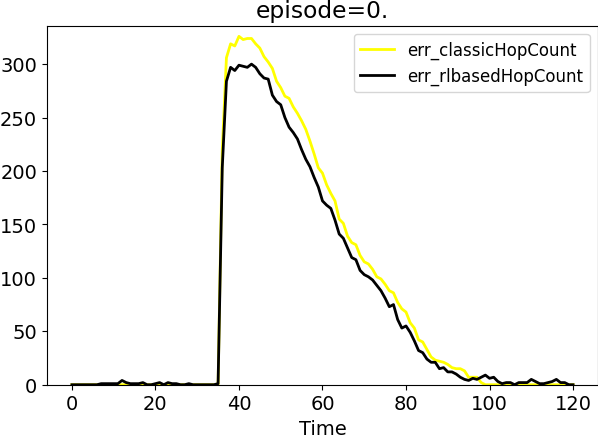
\includegraphics[width=\textwidth]{img/1}
  \end{subfigure}
  \hfill
  \begin{subfigure}[b]{0.3\textwidth}
      \centering
      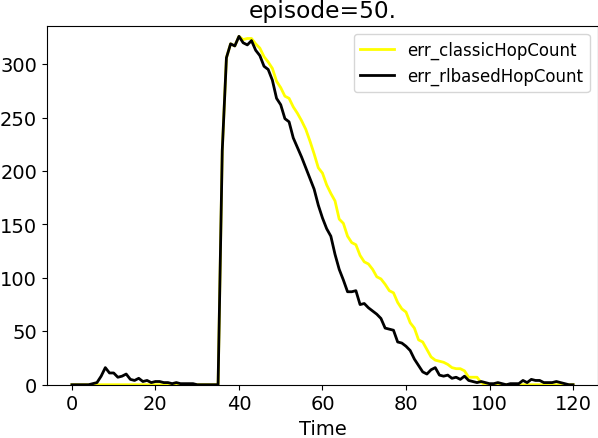
\includegraphics[width=\textwidth]{img/50}
  \end{subfigure}
  \hfill
  \begin{subfigure}[b]{0.3\textwidth}
      \centering
      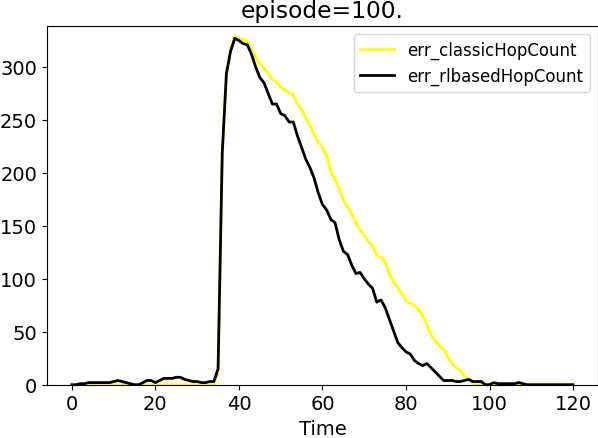
\includegraphics[width=\textwidth]{img/100}
  \end{subfigure}
  \caption{The error evolution compared with naive implementation. The \textit{black} line 
  describes the Reinforcement Learning solution error. The \textit{yellow} line shows
  the naive solution error.}
  \label{fig:simulation}
\end{figure*}
%\todos{add blinking scenarios}
%\todos{add movement scenarios}

\section{Conclusion and Discussion}
In this article, we briefly overview how Aggregate Computing can be mixed with Machine Learning -- 
 in particular with Reinforcement Learning. 
 This leads us to compare Aggregate Computing problems with current Machine Learning solutions in MASs systems.
%
We then define a possible roadmap towards full support of a so-called \hybridaggregate{}, 
 where Machine Learning and Aggregate Computing collaborate.
%
To exemplify how this integration can be performed we build a preliminary use case where 
 learning enhances successfully a standard Aggregate Computing program.


\subsection{Roadmap}
The path towards full integration of Machine Learning and Aggregate Computing is long and probably we do not know the implications that it can bring. 
Currently, we program to:
\begin{enumerate}
  \item Enhance building blocks through learning -- \textit{offline}: 
  in this first step, we need to understand what kind of learning modality is most suitable for us. 
  To decrease the complexity, we aim at perform learning \textit{offline} and at the \textit{building block} level.
  \item Enhance building blocks through learning -- \textit{online}:
  here, the most challenging part in bringing the offline results could be in the reward function definition.
  Indeed, at runtime, we cannot use a global view of the system. 
  A novel way to describe a collective reward by Aggregate Computing might be taken into consideration.
  \item Create building blocks through learning: some building blocks currently lack a proper implementation -- 
  such as the distributed leader election -- so learning can help us also in crafting them. 
  Here, though, the research space increase drastically, 
  so probably it might be not easy to bring our previous results there.
  \item Improve framework aspects through learning: 
  when we successfully apply to learn in the first two steps, 
  we can also consider moving learning at the framework level, to manage non-functional aspects. 
  In this way, developers can focus on the "high level" behaviour aspect.
\end{enumerate}

\todos{discussion about the result}
\todos{limitations: it does not easily scale with the complex application, it cannot be applied online, it cannot be used in different scenarios}
\todos{future work: integrate deep learning solution, integrate actor-critic method (team learning)}
%%
%% Define the bibliography file to be used

\bibliographystyle{IEEEtran}
\bibliography{biblio}
%%
%% If your work has an appendix, this is the place to put it.
%\appendix

\end{document}

%%
%% End of file
